\documentclass[a4paper,11pt,fleqn,twoside,openright,oldfontcommand]{memoir} 	% Openright aabner kapitler paa hoejresider (openany begge)

%%%% PAKKER %%%%

% ¤¤ Oversaettelse og tegnsaetning ¤¤ %
\usepackage[utf8]{inputenc}					% Input-indkodning af tegnsaet (UTF8)
\usepackage[danish]{babel}					% Dokumentets sprog
\usepackage[T1]{fontenc}					% Output-indkodning af tegnsaet (T1)
\usepackage{ragged2e,anyfontsize}			% Justering af elementer
\usepackage{fixltx2e}						% Retter forskellige fejl i LaTeX-kernen
			
																
% ¤¤ Figurer og tabeller (floats) ¤¤ %
\usepackage{graphicx} 						% Haandtering af eksterne billeder (JPG, PNG, PDF)
\usepackage{multirow}                		% Fletning af raekker og kolonner (\multicolumn og \multirow)
\usepackage{colortbl} 						% Farver i tabeller (fx \columncolor, \rowcolor og \cellcolor)
\usepackage[dvipsnames]{xcolor}				% Definer farver med \definecolor. Se mere: http://en.wikibooks.org/wiki/LaTeX/Colors
\usepackage{flafter}						% Soerger for at floats ikke optraeder i teksten foer deres reference
\let\newfloat\relax 						% Justering mellem float-pakken og memoir
\usepackage{float}							% Muliggoer eksakt placering af floats, f.eks. \begin{figure}[H]
%\usepackage{eso-pic}						% Tilfoej billedekommandoer paa hver side
%\usepackage{wrapfig}						% Indsaettelse af figurer omsvoebt af tekst. \begin{wrapfigure}{Placering}{Stoerrelse}
%\usepackage{multicol}         	        	% Muliggoer tekst i spalter
%\usepackage{rotating}						% Rotation af tekst med \begin{sideways}...\end{sideways}

% ¤¤ Matematik mm. ¤¤
\usepackage{amsmath,amssymb,stmaryrd} 		% Avancerede matematik-udvidelser
\usepackage{mathtools}						% Andre matematik- og tegnudvidelser
\usepackage{textcomp}                 		% Symbol-udvidelser (f.eks. promille-tegn med \textperthousand )
\usepackage{siunitx}						% Flot og konsistent praesentation af tal og enheder med \si{enhed} og \SI{tal}{enhed}
\sisetup{output-decimal-marker = {,}}		% Opsaetning af \SI (DE for komma som decimalseparator) 
\usepackage[version=3]{mhchem} 				% Kemi-pakke til flot og let notation af formler, f.eks. \ce{Fe2O3}
%\usepackage{rsphrase}						% Kemi-pakke til RS-saetninger, f.eks. \rsphrase{R1}

% ¤¤ Referencer og kilder ¤¤ %
\usepackage[danish]{varioref}				% Muliggoer bl.a. krydshenvisninger med sidetal (\vref)
\usepackage[numbers,sort&compress]{natbib}

% ¤¤ Misc. ¤¤ %
\usepackage{listings}						% Placer kildekode i dokumentet med \begin{lstlisting}...\end{lstlisting}
\usepackage{lipsum}							% Dummy text \lipsum[..]
\usepackage[shortlabels]{enumitem}			% Muliggoer enkelt konfiguration af lister
\usepackage{pdfpages}						% Goer det muligt at inkludere pdf-dokumenter med kommandoen \includepdf[pages={x-y}]{fil.pdf}	
\pdfoptionpdfminorversion=6					% Muliggoer inkludering af pdf dokumenter, af version 1.6 og hoejere
\pretolerance=2500 							% Justering af afstand mellem ord (hoejt tal, mindre orddeling og mere luft mellem ord)
\usepackage{geometry}
\usepackage{titlesec}  						%needs recent version of »titlesec«
\usepackage{xcolor}

% Kommentarer og rettelser med \fxnote. Med 'final' i stedet for 'draft' udloeser hver note en error i den faerdige rapport.
\usepackage[footnote,draft,danish,silent,nomargin]{fixme}		


%%%% BRUGERDEFINEREDE INDSTILLINGER %%%%

% ¤¤ Marginer ¤¤ %
\setlrmarginsandblock{3.0cm}{3.0cm}{*}		% \setlrmarginsandblock{Indbinding}{Kant}{Ratio}
\setulmarginsandblock{3.0cm}{3.0cm}{*}		% \setulmarginsandblock{Top}{Bund}{Ratio}
\checkandfixthelayout 						% Oversaetter vaerdier til brug for andre pakker

%	¤¤ Afsnitsformatering ¤¤ %
\setlength{\parindent}{0mm}           		% Stoerrelse af indryk
\setlength{\parskip}{3mm}          			% Afstand mellem afsnit ved brug af double Enter
\linespread{1,1}							% Linie afstand

% ¤¤ Litteraturlisten ¤¤ %
\bibliographystyle{unsrtnat}

% ¤¤ Indholdsfortegnelse ¤¤ %
\setsecnumdepth{subsection}		 			% Dybden af nummerede overkrifter (part/chapter/section/subsection)
\maxsecnumdepth{subsection}					% Dokumentklassens graense for nummereringsdybde
\settocdepth{subsection} 					% Dybden af indholdsfortegnelsen

% ¤¤ Lister ¤¤ %
\setlist{
  topsep=0pt,								% Vertikal afstand mellem tekst og listen
  itemsep=-1ex,								% Vertikal afstand mellem items
} 

% ¤¤ Visuelle referencer ¤¤ %
\usepackage[colorlinks]{hyperref}			% Danner klikbare referencer (hyperlinks) i dokumentet.
\hypersetup{colorlinks = true,				% Opsaetning af farvede hyperlinks (interne links, citeringer og URL)
    linkcolor = black,
    citecolor = black,
    urlcolor = black
}

% ¤¤ Opsaetning af figur- og tabeltekst ¤¤ %
\captionnamefont{\small\bfseries\itshape}	% Opsaetning af tekstdelen ('Figur' eller 'Tabel')
\captiontitlefont{\small}					% Opsaetning af nummerering
\captiondelim{. }							% Seperator mellem nummerering og figurtekst
\hangcaption								% Venstrejusterer flere-liniers figurtekst under hinanden
\captionwidth{\linewidth}					% Bredden af figurteksten
\setlength{\belowcaptionskip}{0pt}			% Afstand under figurteksten
		
% ¤¤ Opsaetning af listings ¤¤ %
\definecolor{commentGreen}{RGB}{34,139,24}
\definecolor{stringPurple}{RGB}{208,76,239}

\lstset{language=Matlab,					% Sprog
	basicstyle=\ttfamily\scriptsize,		% Opsaetning af teksten
	keywords={for,if,while,else,elseif,		% Noegleord at fremhaeve
			  end,break,return,case,
			  switch,function},
	keywordstyle=\color{blue},				% Opsaetning af noegleord
	commentstyle=\color{commentGreen},		% Opsaetning af kommentarer
	stringstyle=\color{stringPurple},		% Opsaetning af strenge
	showstringspaces=false,					% Mellemrum i strenge enten vist eller blanke
	numbers=left, numberstyle=\tiny,		% Linjenumre
	extendedchars=true, 					% Tillader specielle karakterer
	columns=flexible,						% Kolonnejustering
	breaklines, breakatwhitespace=true,		% Bryd lange linjer
}

% ¤¤ Navngivning ¤¤ %
\addto\captionsdanish{
	\renewcommand\appendixname{Bilag}
	\renewcommand\contentsname{Indholdsfortegnelse}	
	\renewcommand\appendixpagename{Bilag}
	\renewcommand\appendixtocname{Bilag}
	\renewcommand\cftchaptername{\chaptername~}				% Skriver "Kapitel" foran kapitlerne i indholdsfortegnelsen
	\renewcommand\cftappendixname{\appendixname~}			% Skriver "Appendiks" foran appendiks i indholdsfortegnelsen
}

% ¤¤ Kapiteludssende ¤¤ %
\definecolor{numbercolor}{gray}{0.7}		% Definerer en farve til brug til kapiteludseende
\newif\ifchapternonum

\makechapterstyle{jenor}{					% Definerer kapiteludseende frem til ...
  \renewcommand\beforechapskip{0pt}
  \renewcommand\printchaptername{}
  \renewcommand\printchapternum{}
  \renewcommand\printchapternonum{\chapternonumtrue}
  \renewcommand\chaptitlefont{\fontfamily{pbk}\fontseries{db}\fontshape{n}\fontsize{25}{35}\selectfont\raggedleft}
  \renewcommand\chapnumfont{\fontfamily{pbk}\fontseries{m}\fontshape{n}\fontsize{1in}{0in}\selectfont\color{numbercolor}}
  \renewcommand\printchaptertitle[1]{%
    \noindent
    \ifchapternonum
    \begin{tabularx}{\textwidth}{X}
    {\let\\\newline\chaptitlefont ##1\par} 
    \end{tabularx}
    \par\vskip-2.5mm\hrule
    \else
    \begin{tabularx}{\textwidth}{Xl}
    {\parbox[b]{\linewidth}{\chaptitlefont ##1}} & \raisebox{-15pt}{\chapnumfont \thechapter}
    \end{tabularx}
    \par\vskip2mm\hrule
    \fi
  }
}											% ... her

\chapterstyle{jenor}						% Valg af kapiteludseende - Google 'memoir chapter styles' for alternativer

% ¤¤ Sidehoved/sidefod ¤¤ %

\makepagestyle{Uni}							% Definerer sidehoved og sidefod udseende frem til ...
\makepsmarks{Uni}{%
	\createmark{chapter}{left}{shownumber}{}{. \ }
	\createmark{section}{right}{shownumber}{}{. \ }
	\createplainmark{toc}{both}{\contentsname}
	\createplainmark{lof}{both}{\listfigurename}
	\createplainmark{lot}{both}{\listtablename}
	\createplainmark{bib}{both}{\bibname}
	\createplainmark{index}{both}{\indexname}
	\createplainmark{glossary}{both}{\glossaryname}
}
\nouppercaseheads											% Ingen Caps oenskes

\makeevenhead{Uni}{Gruppe c2-16a}{}{\leftmark}				% Lige siders sidehoved (\makeevenhead{Navn}{Venstre}{Center}{Hoejre})
\makeoddhead{Uni}{\rightmark}{}{Aalborg Universitet}			% Ulige siders sidehoved (\makeoddhead{Navn}{Venstre}{Center}{Hoejre})
\makeevenfoot{Uni}{\thepage}{}{}							% Lige siders sidefod (\makeevenfoot{Navn}{Venstre}{Center}{Hoejre})
\makeoddfoot{Uni}{}{}{\thepage}								% Ulige siders sidefod (\makeoddfoot{Navn}{Venstre}{Center}{Hoejre})
\makeheadrule{Uni}{\textwidth}{0.5pt}						% Tilfoejer en streg under sidehovedets indhold
\makefootrule{Uni}{\textwidth}{0.5pt}{1mm}					% Tilfoejer en streg under sidefodens indhold

\copypagestyle{Unichap}{Uni}								% Sidehoved defineres som blank på kapitelsider
\makeoddhead{Unichap}{}{}{}
\makeevenhead{Unichap}{}{}{}
\makeheadrule{Unichap}{\textwidth}{0pt}
\aliaspagestyle{chapter}{Unichap}							% Den ny style vaelges til at gaelde for chapters
															% ... her
															
\pagestyle{Uni}												% Valg af sidehoved og sidefod (benyt "plain" for ingen sidehoved/fod)


%%%% EGNE KOMMANDOER %%%%

% ¤¤ Billede hack ¤¤ %										% Indsaet figurer nemt med \figur{Stoerrelse}{Fil}{Figurtekst}{Label}
\newcommand{\figur}[4]{
		\begin{figure}[H] \centering
			\includegraphics[width=#1\textwidth]{billeder/#2}
			\caption{#3}
			\label{#4}
		\end{figure} 
}

% ¤¤ Specielle tegn ¤¤ %
\newcommand{\decC}{^{\circ}\text{C}}
\newcommand{\dec}{^{\circ}}
\newcommand{\m}{\cdot}


%%%% ORDDELING %%%%

\hyphenation{In-te-res-se e-le-ment}

%%%% MACRO %%%%

\newenvironment{folderinput}[1]{%
\let\finput\input
\renewcommand{\input}[1]{\finput{#1/##1}}}%
{\let\input\finput}

\raggedbottom
\begin{document}
\thispagestyle{empty}
\begin{flushright}
\vspace{3cm}

\phantom{hul}

\phantom{hul}

\phantom{hul}

\textsl{\Huge Procesanalyse C2-16a} \\ \vspace{1cm}

\rule{13cm}{3mm} \\ \vspace{1.5cm}
\vspace{1cm}

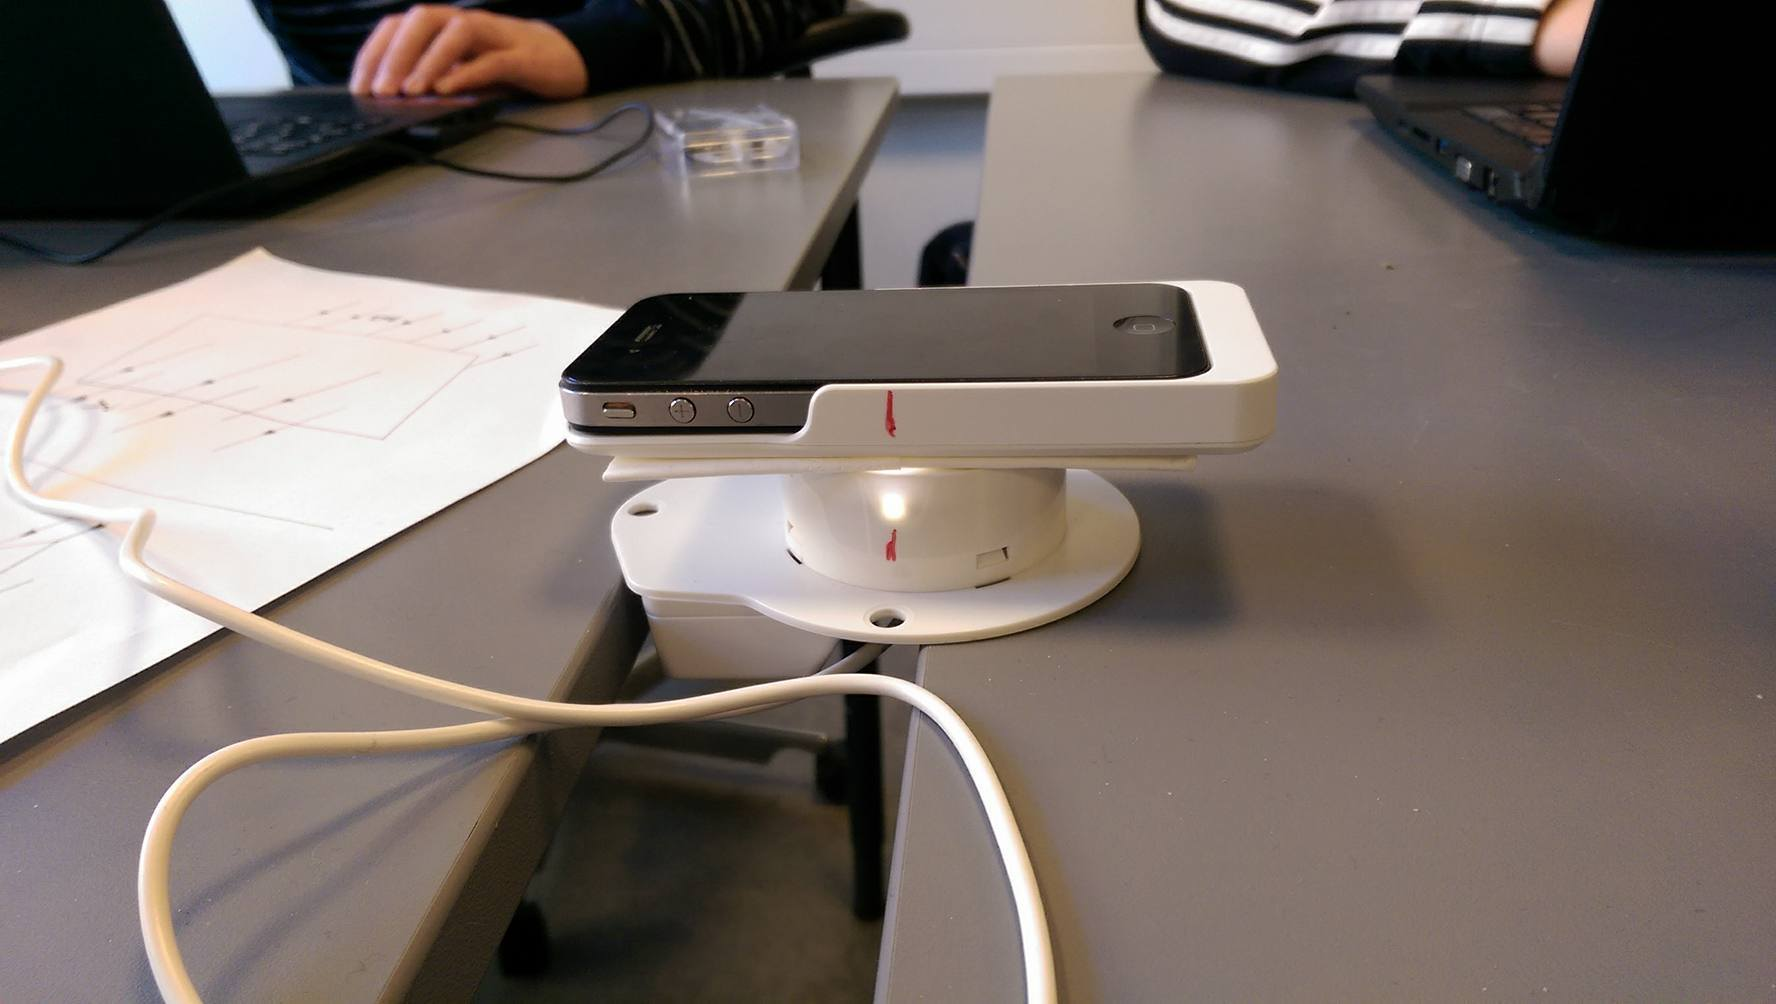
\includegraphics[width=0.864\textwidth]{forsg2_opstilling}

\vspace{2cm} 
\textsc{\Large P1 Projekt \\
Gruppe C2-16a \\
Energi\\
Aalborg Universitet\\
Den 19. december 2016\\}
\end{flushright}

\newpage
\chapter{Processanalyse}
\section{Introduktion}

Formålet med denne processanalyse skal klargøre og reflekterer over gruppen arbejdsindsats gennem projektperioden. Gruppen C2-16a er bestående af Mads Lindstrøm Paulsen, Mathias Stenberg Hansen, Nicolai Nørgaard Munk, Sisse Sorgenfri Jensen, Torben Brund Jørgensen og Daniel Revsbech Pedersen med tilknyttet vejleder Christian Uhrenfeldt. Projektet er forløbet fra 10. oktober 2016 til 21. december 2016. Projekttitel: "Trådløs energioverførsel med fokus på trådløs mobilopladning".

\newpage

%% Table of Contents %%
\phantomsection													% Kunstigt afsnit, som hyperlinks kan 'holde fast i'
\pdfbookmark[0]{Indholdsfortegnelse}{indhold}					% Tildeler en klikbar bookmark til den endelige PDF
\tableofcontents*												% Indholdsfortegnelsen (kaldet ToC)

\newpage

\section{Opstart af projektet}

Gruppen på dannet på baggrund af projektets indhold i forhold til interesse, hvorved medlemmerne blev en sammenfletning af fire forskellige P0-grupper. Ud fra dette grundlag skulle gruppen lære de enkelte individer at kende, hvordan hver enkelt har arbejdet før, og hvilke forventninger der var til projektet. Herudfra skulle gruppen danne et fælles udgangspunkt for, hvad gruppen samlet ville have ud af projektet. Gruppens medlemmer havde forskellige tilgangsformer til projektets start, hvilket skabte en konflikt i starten af projektperioden. For at overkomme denne konflikt skulle der indgås kompromiser for at lave en fælles tilgang til projekts udarbejdning.

Trods gruppens medlemmer kom fra forskellige baggrunde og projekter førhen, så var der en fælles enighed om, at projektet skulle udarbejdes til et tilfredsstillende resultat, uden gruppen forventede topkarakter. Dette gjorde det simpelt at udarbejde en fælles vision for, hvordan gruppen så projektet som helhed, og hvad gruppen samlet gerne ville opnå.

\section{Arbejdsformer}

Ved starten af projektet hvor grundviden skulle indsamles og problemanalysen skulle udarbejdes, så opdelte gruppen sig i mindre grupper for at udvide søgningen efter information. Gruppen gjorde sig hurtigt klart, at alle gruppens medlemmer ikke skulle fokusere på samme område indenfor projektet, hvilket kunne resultere i dobbeltarbejde, hvis alle skrev det samme. Derimod opdelte gruppen sig i mindre arbejdsgrupper på 2-3 personer, som hver havde et emne at fordybe sig i. På denne måde ville flere emner kunne bearbejdes på samme tid, og der skete samtidig en udveksling af nye synspunkter mellem de enkelte gruppers medlemmer, hvilket førte til en mere dybdegående gennemgang af emnerne. 

Ved opdeling i grupperne var det vigtigt, at der var en god kommunikation til sammenfletningen af emnerne. For at alle gruppemedlemmerne havde samme vidensniveau omkring projektet, så blev hele gruppen informeret om, hvis der blev fundet ny viden, som kunne dreje projektet i en anden retning, eller hvis informationerne havde indflydelse på de andre arbejdsgruppers emner. Derudover afholdte gruppen små opsamlinger i løbet af problemanalysen for at gennemgå projektets fremgang og dele ny viden.

Til udarbejdningen af problemformuleringen gennemgik gruppen den indsamlede viden omkring projektet i forbindelse med problemanalysen. Derved havde gruppen en fælles forståelse og forudsætning for at opsætte en beskrivende problemformulering. Hvert gruppemedlem skulle opsætte tre bud på en problemformulering, hvorefter alle buddene blev fremlagt for resten af gruppen. Alle formuleringer blev taget i betragtning, hvorved gruppen samlet kunne benytte forslagene til at opsætte en kort og præcis formulering i fællesskab.

Til vidensdeling af forsøg, benyttede gruppen sig af, at der var 2-3 stykker som gik i laboratorie, for at lave forsøgende, imens resten af gruppen lavede videre på teoristykket, som viderebygning til forsøgende. Dem som ikke fik en praktik viden af forsøgende, lavede sig en teoretisk forståelse for forsøgendes udførelse. Til vidensdeling af dokumenter brugte gruppen \textit{SmartGit}, gennem dette program kunne gruppen dele dokumenterne, og der kunne laves et fælles dokument for projektet, hvor flere af gruppen medlemmer kunne skrive i på samme tid.

Mod slutning af projektet blev de resterende opgaver ført på tavlen, og herudfra kunne gruppe medlemmerne sætte sig på en af disse opgave. Der blev også ført en dagsorden på tavlen, så gruppen kunne se og følge med i, hvad der blev/skulle laves færdig for dagen. Hvis et emne førte til videre arbejde, så blev dette punkt skrevet på tavlen, hvorved andre kunne hjælpe til og få en forståelse af indholdet i projektet. 

Gennem hele projektet har gruppen benyttet sig af samarbejde med vejleder, til en dybere forståelse og indsigt i projektet. Vejleder havde igennem projektet forslag til forsøg og emner, hvis gruppen selv var gået i stå. Vejleder var også behjælpelig med svar på teoretiske spørgsmål, og hjælp til opbygning af projektet.  Gruppen var lidt tilbageholdt med at benytte vejlederen, og fandt hurtigt ud af, at han var der for at hjælpe med alt. Mod slutningen af projektet kom der en forståelse for gruppen, at flere møder med vejlederen ville have gavnet projektets forløb.

\section{Projektplanlægning og -styring}

Som gruppe er det vigtigt af have en ens tankegang for ikke at skabe flere konflikter end nødvendigt. Til at opsætte fælles retningslinjer for gruppens medlemmer, så blev der udarbejdet en gruppekontrakt eller arbejdsaftale, som alle medlemmer af gruppen kunne stå inde for. Gruppekontrakten fastslog en fast mødetid for projektarbejdet. Hvis et medlem i gruppen først kunne møde senere, eller de af en årsag måtte tage en skrivedag hjemme, så skulle dette informeres til gruppe inden mødetid (og gerne dagen før), ellers ville personen skylde morgenbrød eller lignende. Derudover indeholdte kontrakten et krav til alle medlemmer om, at alle skulle yde en indsats og møde velforberedte op, så der ikke gik spildtid med at informere andre gruppemedlemmer. Gruppekontrakten opstillede også retningslinjer til, hvordan projektet kunne holdes struktureret ved brug af en tidsplan og en logbog over projektets fremgang. (Se bilag 1)

Gruppen fik opsat gruppekontrakten et par uger inde i selve projektet, og den blev ikke udspecificeret nok, hvilket gjorde at den ikke blev overholdt. Der var heller ikke påsat et gruppemedlem til at styre gruppekontrakten og sørge for, at den blev overhold, så det resulterede i, at gruppekontrakten ikke var gældende for projektets forløb. Dette gav komplikationer i forbindelse med, at der opstod en sløset kultur for mødetider, og strukturen i projektet var ikke så velorganiseret som håbet. Dette havde en skadelig effekt på gruppen og resulterede i, at der opstod stress og tidspres ved slutningen af projektet.

Ved opstarten af projektet blev der opsat en grov tidsplan over problemanalysen, hvor der stod beskrevet, hvornår de enkelte arbejdsmål og selve problemanalysen skulle afsluttes, samt hvilke medlemmer der stod for hver del. Til dette benyttede gruppen et program kaldet \textit{GanttProject} (Se bilag 2), hvor arbejdet kunne koordineres fra. Mod slutningen af problemanalysen skulle tidsplanen ændres, men dette gik i glemmebogen, hvorefter det ikke blev genoptaget ved resten af projektet.

Da der ikke var nogle medlemmer påsat til at styre hverken gruppekontrakten eller tidsplanen, så mistede gruppen fokus fra dette, og det forsvandt til sidst ud af projektet. Derved kunne gruppen med fordel have benyttet sig af grupperoller for inddeling af arbejdet, så hvert medlem fik et fokusområde, de kunne opretholde. Til gengæld indfandt de enkelte medlemmer sig i forskellige roller gennem projektet, hvilket skabte et mere naturligt sammenspil i gruppen, end hvis rollerne var påtvunget.

Ved at tidsplanen og gruppesammenspillet ikke rigtig var i top mod slutningen af projektet, så blev gruppen stresset, da der var rigeligt, som skulle skrives endnu og ikke rigtig tid til det hele. Gruppen håndterede denne periode ved, at sætte deres fokus på de punkter, som var bagud i tidsplanen, og derved kunne gruppen ikke komme ind på andre emner i projektet. Gruppen var for længe i "Paniczone", og fik ikke rigtig styr på deres emner, og der blev for meget at skrive til sidst. For at overkomme problemet med de haltende emner, indførte gruppen delmål for hvert emne, hvem der skulle gøre det færdigt, og hvornår det skulle være klar. Derved blev de resterende punkter bearbejdet og beskrevet. Igennem projektperioden opstod der flere konflikter for gruppen, ca. en måned inde i projektet valgte et gruppemedlem at hoppe fra uddannelsen, og dette betød at gruppen var en mand mindre, gruppen prøvede at komme i kontakt med personen, men dette lykkesede ikke. Gruppen valgte at vente i et par uger til at se, om personen selv kontaktede skolen og meldte sit fravær, men da dette ikke skete, kontaktede gruppen vejleder, og holdte et møde, for at kunne snakke om, hvad der skulle ske. Gruppen skulle have været bedre til, at sige fra og få fat i vejlederen noget tidligere og få personen helt ud af gruppen hurtigt. Derudover opstod der konflikt med en persons entusiasme for projektet, og personen valgte ikke at møde op længere. Der skulle gruppen have været kontant og have taget det op ved næste vejleder møde, så der kunne have været fundet en løsning på dette. Gruppen skulle derfor have været bedre til konfliktløsning, og taget problemet op med det samme, og fået snakket det igennem, denne tanke tager gruppen med sig videre. 

\section{Læringsprocess}

For håndtering af dokumenter har gruppen hovedsageligt været gode til at dele nye eller opdaterede dele af projektet med hinanden. Til deling af dokumenter benyttede gruppen programmet SmartGit, hvor hvert medlem kunne indsende sine egne dokumenter eller rettelser i dokumenter, men også hente andre gruppemedlemmers dokumenter ned, så alle havde de opdaterede dele af rapporten. Gruppen stødte dog på det problem, at gruppemedlemmet, der mistede entusiasmen for projektet, ikke satte sig ind i programmet, trods resten af gruppen hjalp personen. Derved modtog gruppen tekstdokumenter fra den sidste person, som derefter skulle indskrives i det rette program. Til at gemme og håndtere kilder har gruppen benyttet sig af programmet Mendeley, hvor kilden kan uploades til med forfatter, udgivelsesår o.s.v. Herved har alle haft adgang til hinandens kilder, og de let kunne implementeres i rapporten.

Gennem projektet er der benyttet forskellige kvantitative metoder til indsamling af data og resultater. Først benyttede gruppen kvantitativ metode i forbindelse med simulationer af de elektriske kredsløb. Derudover er den kvantitative metode benyttet til udførelsen af forsøgene med de elektriske kredsløb, hvor der også her blev indsamlet en masse resultater, som senere er blevet beregnet på og indsat i grafer, som kan benyttes til sammenligning med de andre forsøg.

Til projektet er der benyttet kilder i forskellig form. Hovedsageligt er der benyttet videnskabelige artikler eller fagværker, som er godkendt af AAU's bibliotek eller i mindste fald scholar.google.dk. For andre kilder, som brugt til personers historiske baggrund, er der benyttet online biografier eller gyldendals hjemmeside, som er gennemgået af tjek. De videnskabelige artikler er angivet med en forfatter, som kan undersøges for troværdighed.

\newpage

\section{Reflektion over projektet}

P1-projektet har dannet baggrund for en god mængde erfaringer til fremadrettede projekter. Gruppemedlemmerne har modtaget et billede på, hvad der fungerede i gruppearbejdet, hvad der kunne forbedres, og hvad der ikke skal benyttes til næste projekt. For gruppens tilfælde er der kommet en forståelse for, at store beslutninger for gruppens vedkommende ikke skal trækkes i langdrag, men skal håndteres med det samme. Her er der bl.a. tanke på eksklusionen af et gruppemedlem, som meldte ud, at personen ikke længere deltager, men ikke informerede universitetet omkring vedkommendes afgang. Derudover har projektet været en øjenåbner for nødvendigheden af struktur gennem processen. Her kan der f.eks. tænkes på at sætte ansvarlige på hver opgave, så der bliver taget hånd omkring opgaven fremfor, at hjælpemidlet går tabt. Her tænkes der på gruppens gruppekontrakt og tidsplan. I forlængelse af dette er det nødvendigt at benytte hjælpemidler fra starten, og ikke når der er gået flere uger, så det bliver gjort og kan benyttes.

Hvad gruppen kan tage videre med sig fra projektet er bl.a. uddelingen af arbejdsgrupper, som benyttet i problemanalysen, hvor arbejdet blev fordelt i grupper på 2-3 personer, hvilket fordeler arbejdsbyrden. På denne måde sidder der ikke for mange omkring samme emne, men samtidig bliver opgaven ikke præget af individuelt arbejde, så der stadig kommer forskellige synspunkter på hvert emne. Derudover kan brugen af forsøg tages videre til senere projekter, hvilket er med til at give en bedre forståelse for projektets sammenhæng. Gennem forsøg skabes der en visuel forståelse, som kan lægges i forlængelse af den teoretiske viden opbygget gennem rapporten.

Hurtigere i gang med sociale arrangementer og flere af dem. Dette er noget gruppen har opdaget da det ikke var noget der blev brugt megen tid på. Normalt er dette noget som institutionen arrangere for de studerene, som i P0, men sådanne kan det jo ikke blive ved med at være. Det er tydeligt at man først ved hvad man har når man ikke længere har det mere. Altså det er tydeligt at arrangementer i en gruppe kan have en stor effekt. Denne effekt er på det sociale sammenhold i gruppen, specielt hvis man er syv mennesker der ikke kender hinanden og kommer fra vidt forskellige bagrunde. Dette sociale sammenhold der dannes gennem arrangementer kan have en direkte effekt på det faglige som i sidste ende er det vigtigste på universitetet. Dette er måske ikke sandt for alle i gruppen, alle er jo forskellige men hvis det kan hjælpe nogen i gruppen styrker det gruppen i det hele.

\section{Konklusion}

Gruppen har igennem dette projekt lært, at det er en fælles indsats, og det er ikke et individuelt arbejde, for at få en projekt færdig. Det er vigtigt for gruppearbejdet, at der i starten af projektperioden dannes tillid og respekt til hinanden, hvilket også betyder, at man skal sige, hvis man er bagud eller det er svært. Det er vigtigt, at hjælpe hinanden, hvis et gruppemedlem går i stå. Det er også vigtigt, at hvert gruppemedlem er indforstået med arbejdet, og de fælles mål for projektet, og at der bliver overholdt tidsplaner.
Gruppen har også lært, at tidsplaner er utrolig vigtige, og det gælder om at få dem lavet tidligt, og få dem opdateret igennem projektperioden. Så det ikke ender ud i, at man sidder den sidste uge og skal skrive et hel projekt. Indvidere er det vigtigt, at man indskrænker kilder og viden tidligt i projektperioden, så der ikke bruges 2 uger på, at læser kilder, som slet ikke skal benyttes. Gruppen skal derfor være bedre til, at håndtere kilder, altså kassere dem som ikke skal benyttes.

\chapter{Bilag}

\begin{figure} [H]
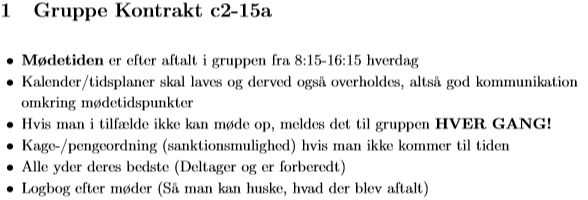
\includegraphics[scale=1]{Gruppekontrakt}
\caption{Gruppekontakt}
\end{figure}

\begin{figure} [H]
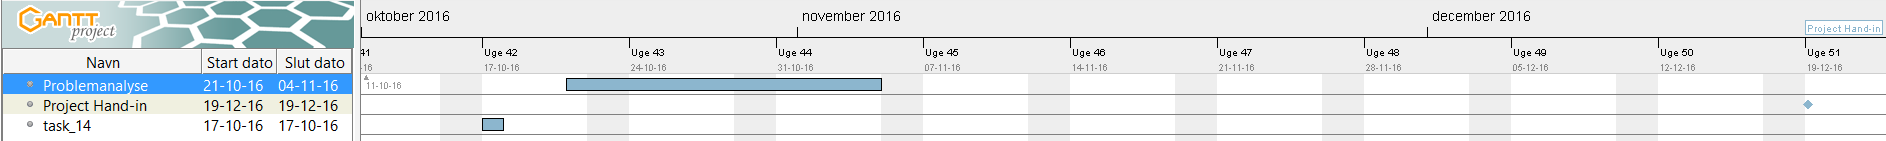
\includegraphics[scale=0.35]{Tidsplan1}
\caption{Tidsplan}
\end{figure}

\begin{figure} [H]
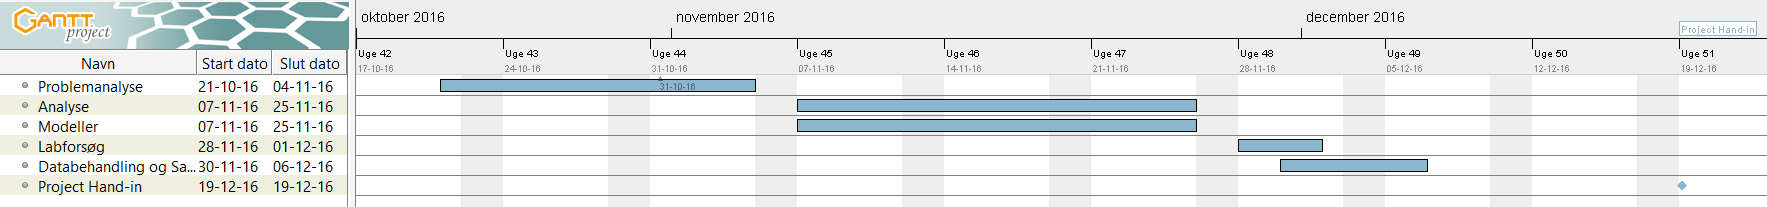
\includegraphics[scale=0.35]{Tidsplan2}
\caption{Tidsplan}
\end{figure}

\end{document}